\newpage 

\section{Cost of Electricity} 

 Contributors to LCOE projections are given by: 
 \begin{equation} 
 LCOE [\$ MWh] = \frac{(C_{AC} + (C_{OM} + C_{F})(1+y)^Y)}{(8760.P_E.p_a)} 
 \label{eq:coe}
\end{equation} 
where C$_{AC}$ [USD/year] is the annual capital cost charge (entailing the total capital cost of the plant (TCC (USD) multiplied by the Fixed Charge Rate (FCR (/year)), C$_{OM}$ [USD/year] is the annual operations and maintenance cost, C$_{SCR}$ [USD/year] is the annual scheduled component replacement costs, C$_{F}$ [USD/year] is the annual fuel costs, $y$ is the annual fractional increase in fuel costs over the expected lifetime of the plant $Y$ [years], P$_{E}$ [MWe] is the electric power of the plant, p$_{a}$ is the plant availability (typically 0.6-0.9).  A small charge used to be imposed to build up a fund to cover end-of-life Decontamination and Decommissioning, f$_{DD}$ (USD/kWh).  The Decommissioning costs are now included in the direct capitalized costs (Cost Category 58), so are omitted here.


% \subsection{Cost Category 70: Annualized O\&M Cost (AOC)}

The Operations and Maintenance (O\&M) costs was previously estimated to be 2 \% of the direct cost, assessed annually.  The O\&M cost depends on the system complexity and the requirements of regulations, security and maintenance. The costs are computed based on look-up tables, such as the one shown in Fig. \ref{fig:statista} at 60 USD per kilowatt-year.  

\begin{figure}[b!] 
\centering 
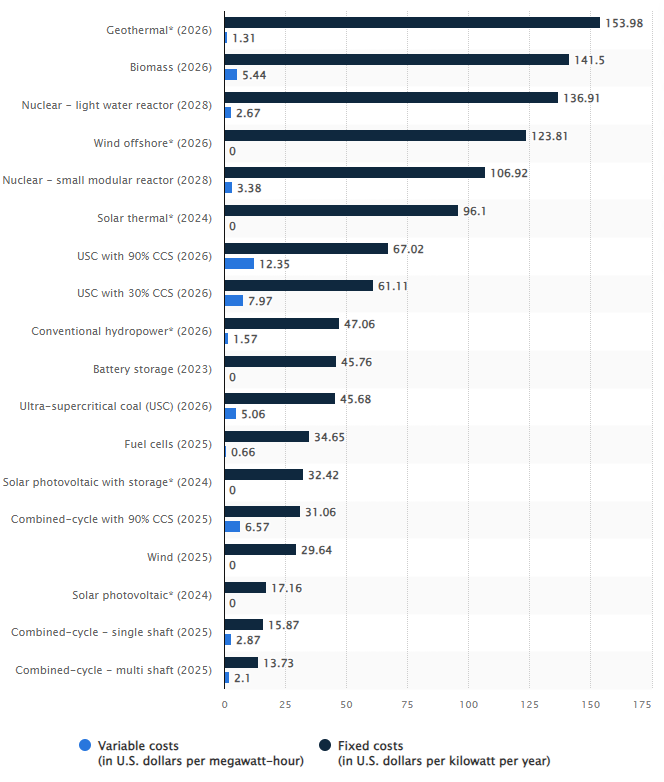
\includegraphics[scale=0.5]{StandardFigures/statista.png} 
\caption{Operations and Maintenance costs for various kinds of power plants.} 
\label{fig:statista} 
\end{figure} 

\begin{verbatim} 
C_OM = 60 * PE * 1000 = C700000  
\end{verbatim} 

Annualized O\&M costs are \$ C700000 M.

\subsubsection*{Cost Category 71 – O\&M Staff}
This Cost Category includes salary costs of O\&M staff.

\subsubsection*{Cost Category 72 – Management Staff}
This Cost Category includes salary costs of operations management staff.

\subsubsection*{Cost Category 73 – Salary-Related Costs}
This Cost Category includes taxes, insurance, fringes, benefits, and any other annual salary-related costs.

\subsubsection*{Cost Category 74 – Operations Chemicals, and Lubricants}

\subsubsection*{Cost Category 75 – Spare Parts}
Cost of any operational spare parts, excluding capital plant upgrades or major equipment that will be capitalized or amortized over some period or quantity of product.\\

Annual Scheduled Replacement Cost. The cost of scheduled component replacement is now included in the annual operations and maintenance charge.  Here we assume that the components in the first wall and the blanket are replaced every 10 years, giving an annual replacement cost of \$ C750000 M.


\subsubsection*{Cost Category 76 – Utilities, Supplies, and Consumables}
Cost of water, gas, electricity, tools, machinery, maintenance equipment, office supplies and similar items purchased annually.

\subsubsection*{Cost Category 77 – Capital Plant Upgrades}
Upgrades to maintain or improve plant capacity, meet future regulatory requirements or plant life extensions.

\subsubsection*{Cost Category 78 – Taxes and Insurance}
Property taxes and insurance costs, excluding salary related.

\subsubsection*{Cost Category 79 – Contingency on Annualized O\&M Costs}
This Cost Category includes an assessment of additional cost necessary to achieve the desired confidence level for the annualized O\&M costs not to be exceeded.

% \subsection{Cost Category 80: Annualized Fuel Cost (AFC)}

%\subsection{Annual Fuel Cost} 
The fuel cost, C$_{F}$, is calculated as follows.  The unit cost of deuterium as D2 is 3,700 \$/kg; deuterium contributes negligibly to the COE of a fusion power plant. In the long run, the power plant is self-sufficient in terms of tritium fuel production because of the breeding capability of the blanket so that no specific tritium-fuel charge is reported. It should be recognized, however, that there is a significant cost for tritium in the direct cost of the D-T fueled fusion reactor, represented in Cost Category 22.5 Fuel Handling and Storage. Cost of the lead lithium materials is included in Cost Category 27 Special Materials.\\

Consists of:  
\begin{verbatim} 
m_D = 3.342*10^(-27) # (kg)
u_D = 2175 #Where u_D ($/kg) = 2175 ($/kg) 
C_F = N_mod * P_NRL * 1e6 * 3600 * 8760 * u_D * m_D * p_a / (17.58 * 1.6021e-13)
\end{verbatim} 

Total annual fuel costs are \$ C800000 M per year.

\subsubsection*{Cost Category 81 – Refueling Operations}
This Cost Category includes incremental costs associated with refueling operations.

\subsubsection*{Cost Category 84 – Fuel}
This Cost Category includes annualized costs associated with the fuel cycle.

\subsubsection*{Cost Category 86 – Processing Charges}
This Cost Category includes storage and processing if fuel is brought in from offsite.

\subsubsection*{Cost Category 87 – Special Nuclear Materials}
This Cost Category covers materials such as heavy water, sodium, lead, helium, or other energy transfer mediums that are required on an annual basis. It includes costs associated with disposal or treatment if necessary. 

\subsubsection*{Cost Category 89 – Contingency on Annualized Fuel Costs}
This Cost Category includes an assessment of additional cost necessary to achieve the desired confidence level for the annualized fuel costs not to be exceeded.

% \subsection{Cost Category 90: Annualized Financial Costs (AFC)}

Consists of: Capital return factor (or constant dollar FCR), $f_{cr}$ multiplied by the total capital cost. FCR calculation follows the methods outlined by the 2019 NETL report \cite{NETL2019a}.

\begin{verbatim} 
f_cr = 0.074 
C_AC (USD/year) = f_cr * C_99*1e6 = 274872277.2
\end{verbatim} 

Annualized Financial Costs are \$ C900000 M.

\subsubsection*{Account 91 – Escalation}
This account is excluded from estimated costs, although it could be included in a business plan, a financing proposal, or regulatory-related documents.

\subsubsection*{Account 92 – Fees}
Cost of fees incurred for annual fees such as licensed reactor process, nuclear operating license fees, and similar.

\subsubsection*{Account 93 – Cost of Money}
Value of money utilized for operating costs. May be financed externally or retained earnings.

\subsubsection*{Account 99 – Contingency on Annualized Financial Costs}
This account includes an assessment of additional costs necessary to achieve the desired confidence level for the annualized financial costs not to be exceeded, including schedule uncertainties.


\subsection{Cost Category 70: Annualized O\&M Cost (AOC)}

The Operations and Maintenance (O\&M) costs was previously estimated to be 2 \% of the direct cost, assessed annually.  The O\&M cost depends on the system complexity and the requirements of regulations, security and maintenance. The costs are computed based on look-up tables, such as the one shown in Fig. \ref{fig:statista} at 60 USD per kilowatt-year.  

\begin{figure}[b!] 
\centering 
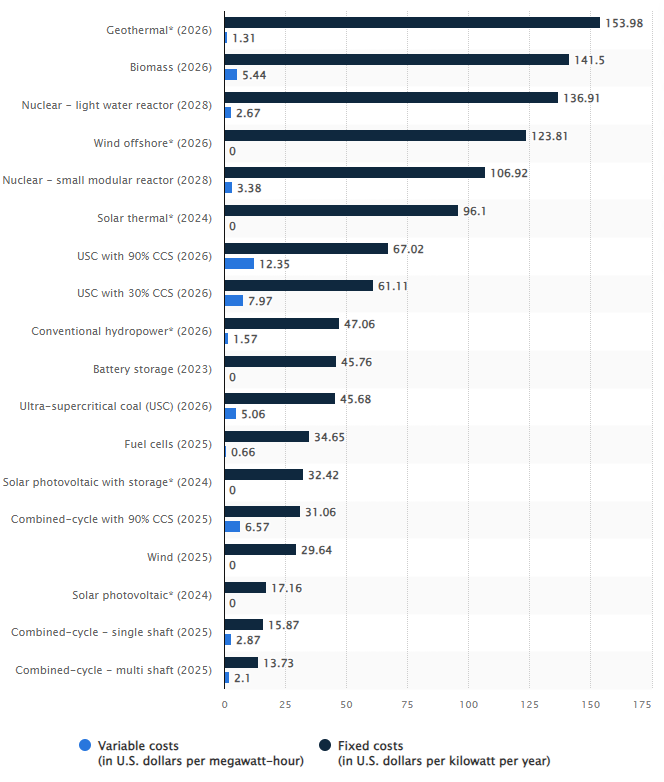
\includegraphics[scale=0.5]{StandardFigures/statista.png} 
\caption{Operations and Maintenance costs for various kinds of power plants.} 
\label{fig:statista} 
\end{figure} 

\begin{verbatim} 
C_OM = 60 * PE * 1000 = C700000  
\end{verbatim} 

Annualized O\&M costs are \$ C700000 M.

\subsubsection*{Cost Category 71 – O\&M Staff}
This Cost Category includes salary costs of O\&M staff.

\subsubsection*{Cost Category 72 – Management Staff}
This Cost Category includes salary costs of operations management staff.

\subsubsection*{Cost Category 73 – Salary-Related Costs}
This Cost Category includes taxes, insurance, fringes, benefits, and any other annual salary-related costs.

\subsubsection*{Cost Category 74 – Operations Chemicals, and Lubricants}

\subsubsection*{Cost Category 75 – Spare Parts}
Cost of any operational spare parts, excluding capital plant upgrades or major equipment that will be capitalized or amortized over some period or quantity of product.\\

Annual Scheduled Replacement Cost. The cost of scheduled component replacement is now included in the annual operations and maintenance charge.  Here we assume that the components in the first wall and the blanket are replaced every 10 years, giving an annual replacement cost of \$ C750000 M.


\subsubsection*{Cost Category 76 – Utilities, Supplies, and Consumables}
Cost of water, gas, electricity, tools, machinery, maintenance equipment, office supplies and similar items purchased annually.

\subsubsection*{Cost Category 77 – Capital Plant Upgrades}
Upgrades to maintain or improve plant capacity, meet future regulatory requirements or plant life extensions.

\subsubsection*{Cost Category 78 – Taxes and Insurance}
Property taxes and insurance costs, excluding salary related.

\subsubsection*{Cost Category 79 – Contingency on Annualized O\&M Costs}
This Cost Category includes an assessment of additional cost necessary to achieve the desired confidence level for the annualized O\&M costs not to be exceeded.

\subsection{Cost Category 80: Annualized Fuel Cost (AFC)}

%\subsection{Annual Fuel Cost} 
The fuel cost, C$_{F}$, is calculated as follows.  The unit cost of deuterium as D2 is 3,700 \$/kg; deuterium contributes negligibly to the COE of a fusion power plant. In the long run, the power plant is self-sufficient in terms of tritium fuel production because of the breeding capability of the blanket so that no specific tritium-fuel charge is reported. It should be recognized, however, that there is a significant cost for tritium in the direct cost of the D-T fueled fusion reactor, represented in Cost Category 22.5 Fuel Handling and Storage. Cost of the lead lithium materials is included in Cost Category 27 Special Materials.\\

Consists of:  
\begin{verbatim} 
m_D = 3.342*10^(-27) # (kg)
u_D = 2175 #Where u_D ($/kg) = 2175 ($/kg) 
C_F = N_mod * P_NRL * 1e6 * 3600 * 8760 * u_D * m_D * p_a / (17.58 * 1.6021e-13)
\end{verbatim} 

Total annual fuel costs are \$ C800000 M per year.

\subsubsection*{Cost Category 81 – Refueling Operations}
This Cost Category includes incremental costs associated with refueling operations.

\subsubsection*{Cost Category 84 – Fuel}
This Cost Category includes annualized costs associated with the fuel cycle.

\subsubsection*{Cost Category 86 – Processing Charges}
This Cost Category includes storage and processing if fuel is brought in from offsite.

\subsubsection*{Cost Category 87 – Special Nuclear Materials}
This Cost Category covers materials such as heavy water, sodium, lead, helium, or other energy transfer mediums that are required on an annual basis. It includes costs associated with disposal or treatment if necessary. 

\subsubsection*{Cost Category 89 – Contingency on Annualized Fuel Costs}
This Cost Category includes an assessment of additional cost necessary to achieve the desired confidence level for the annualized fuel costs not to be exceeded.

\subsection{Cost Category 90: Annualized Financial Costs (AFC)}

Consists of: Capital return factor (or constant dollar FCR), $f_{cr}$ multiplied by the total capital cost. FCR calculation follows the methods outlined by the 2019 NETL report \cite{NETL2019a}.

\begin{verbatim} 
f_cr = 0.074 
C_AC (USD/year) = f_cr * C_99*1e6 = 274872277.2
\end{verbatim} 

Annualized Financial Costs are \$ C900000 M.

\subsubsection*{Account 91 – Escalation}
This account is excluded from estimated costs, although it could be included in a business plan, a financing proposal, or regulatory-related documents.

\subsubsection*{Account 92 – Fees}
Cost of fees incurred for annual fees such as licensed reactor process, nuclear operating license fees, and similar.

\subsubsection*{Account 93 – Cost of Money}
Value of money utilized for operating costs. May be financed externally or retained earnings.

\subsubsection*{Account 99 – Contingency on Annualized Financial Costs}
This account includes an assessment of additional costs necessary to achieve the desired confidence level for the annualized financial costs not to be exceeded, including schedule uncertainties.


\subsection{Levelized Cost of Electricity} 

\begin{table}[h!] 
\begin{tabular}{l c c } 
Capital cost, $C_{AC}$ &     M\$/annum    &    C900000      \\ 
Scheduled Replacement Costs, $C_{SCR}$  &     M\$/annum    &  C750000   \\ 
Operations and Maintenance Costs, $C_{OM}$ & M\$/annum  &      C700000 \\ 
Fuel Costs, $C_{F}$ & M\$/annum  &       C800000 \\ 
    \end{tabular} 
    \caption{Cost components in the LCOE calcualtion.}
    \label{tab:lcoe} 
\end{table} 

Following equation \ref{eq:coe}, the LCOE is C1000000 \$/MWh or C2000000 c/kWh. 

%\subsection{Levelized Cost of Electricity Nth of a Kind (NOAK)}  

%It is possible to distinguish between the First of a Kind (FOAK) power plant, which might function as a Demo, and more mature 10th of a Kind (TOAK), the latter incorporating learning credits in the COE estimate, consistent with U.S. fusion-reactor design-community practice. The ARIES study, like STARFIRE \cite{BAK80} and most other U.S. fusion-reactor designs reported in the last decade, assumes FPC unit costs consistent with these learning-curve \cite{Hir64,Arg90} credits, rather than first-of-a-kind unit costs (including R\&D) appropriate for ITER \cite{Ite89} or some other reported designs \cite{Coo89b}. An 80 \% learning curve ({\it {\it i.e.},} 0.80 progress ratio, $p$), as used for ARIES, represents the expectation that each doubling of production represents a \hbox{$p\simeq$ 0.8} reduction in unit costs. A tenth-of-a-kind reactor represents, nominally, $\simeq$3.3 doubling of production or $p^{(ln 10/ln 2)}\simeq$ 50 \% cost reduction relative to first-of-a-kind FPC costs.  Of course, the actual production experience varies \cite{Arg90}.  Learning credits are not applied to BOP items, consistent with mature industrial production in which the learning credits have already been wrung out.  For similar reasons, a 94 \% learning curve is recommended for advanced fission cost estimates \cite{Del93}.   